\documentclass[11pt,a4paper]{article}
\usepackage[T1]{fontenc}
\usepackage{lmodern,amsmath,amssymb,amsthm,mathtools}
\usepackage[margin=25mm,headheight=15pt]{geometry}
\usepackage{graphicx,booktabs,array,tabularx,longtable}
\usepackage[dvipsnames]{xcolor}
\usepackage{microtype,enumitem,fancyhdr,needspace}
\usepackage[colorlinks=true,linkcolor=MidnightBlue,citecolor=MidnightBlue,urlcolor=MidnightBlue]{hyperref}
\usepackage{bookmark}
\hypersetup{pdftitle={Central-Route Accounting and Six-Opening Geometry in the Reciprocal Chiral Exchange Candidate},pdfauthor={Hilmir Frímann Halldórsson (pzychozen)},pdfsubject={Research edition v0.1 — accepted mathematics; author-authorized repository publication},pdfkeywords={reciprocal exchange, central-route accounting, six-opening geometry, 10 November 2026}}
\setlength{\parindent}{0pt}
\setlength{\parskip}{4pt}
\setlength{\emergencystretch}{3em}
\setlist{nosep,leftmargin=*}
\numberwithin{equation}{section}
\newtheorem{theorem}{Theorem}[section]
\newtheorem{proposition}[theorem]{Proposition}
\newtheorem{corollary}[theorem]{Corollary}
\theoremstyle{remark}\newtheorem{remark}[theorem]{Remark}
\newcommand{\R}{\mathbb R}
\newcommand{\C}{\mathbb C}
\newcommand{\norm}[1]{\left\lVert#1\right\rVert}
\newcommand{\abs}[1]{\left|#1\right|}
\newcommand{\Sb}{\mathcal S_b}
\newcommand{\Hull}{\mathcal H}
\newcommand{\dd}{\,\mathrm d}
\newcommand{\ee}{e_z}
\newcommand{\rc}{r_c}
\newcommand{\epsc}{\epsilon_c}
\newcommand{\RG}{R_\Gamma}
\newcommand{\Gain}{G_{\rm gain}}
\newcommand{\wh}{w_{\rm host}}
\newcommand{\sourcepath}[1]{\texttt{\detokenize{#1}}}
\pagestyle{fancy}\fancyhf{}
\fancyhead[L]{\small Central-route accounting and six-opening geometry}
\fancyhead[R]{\small v0.1}
\fancyfoot[C]{\thepage}
\begin{document}
\hypersetup{pageanchor=false}
\begin{titlepage}
\centering
\vspace*{17mm}
{\LARGE\bfseries Central-Route Accounting and\\[3mm] Six-Opening Geometry in the\\[3mm] Reciprocal Chiral Exchange Candidate\par}
\vspace{11mm}
{\large Hilmir Frímann Halldórsson (pzychozen)\par}
\vspace{4mm}
{10 November 2026\par}
\vspace{5mm}
{\small Research edition v0.1\par
Accepted mathematics; author-authorized repository publication\par}
\vspace{10mm}
\begin{minipage}{0.94\textwidth}
\textbf{Abstract.}
The reciprocal chiral exchange candidate couples a native state to a spatially registered periodic carrier and a reversible receiver through finite profiles. We examine what its exact work account establishes about an intended outward--around--inward route. For empty carrier and receiver preparation, positive couplings and a nonzero registered drive, receiver storage grows at quartic order while the nearest carrier point to the central origin remains inactive. Diagnostic cuts strictly enclosing both source profiles also remain inactive initially. We derive the regional account, including complementary-profile work and native jumps, and give the full cut-distance criterion, which also permits delayed inner cuts. Independently, a scalar separator proves that all three inherited geometric circles are uniformly separated from each of the six central opening boundaries and its individual convex enclosure, throughout the admitted static geometry family and for both hands. The distance exceeds $297/5000$ times the common host width. These enclosures are mathematical bounds, not adopted apertures. Thus the existing host contacts cannot be relabeled as direct central-opening crossings; an undefined physical aperture flux has not been computed as zero. Common-phase symmetry further limits what exchange histories alone can recover about a phase-sensitive outlet. The paper identifies the additional spatial and work registration needed to relate the demonstrated exchange to a larger transport circuit.
\end{minipage}
\vfill
\begin{minipage}{0.94\textwidth}\small
\textbf{Preparation and status.} Hilmir Frímann Halldórsson provides authorship and geometric direction. GPT contributed formulation and project-internal mathematical review; Codex performed the independent investigations and manuscript preparation. The accepted central-route results include qualification Q01, and the six-opening results are accepted as stated. This edition is an author-authorized repository research publication. The accompanying review and correction records state the scope of project-internal review; no external peer review or formally verified proof is claimed.
\end{minipage}
\end{titlepage}
\hypersetup{pageanchor=true}\setcounter{page}{2}
\section{Question and principal results}\label{sec:question}
The geometric motivation is a central starting or meeting region, opposed upward and downward routes, outward spreading and a curved return, possibly with transfer elsewhere, while the native supports remain stationary. A correspondence argument must connect that picture to the actual state variables and exchange laws. Storage gained by a receiver is an energetic statement; crossing a specified spatial boundary is a separate geometric and dynamical statement.

The inherited candidate already supplies substantial structure: positioned native support lines, a registered carrier curve with two finite host contacts, reciprocal native feedback, a reversible receiver and a matched work account \cite{AX,CC,RX,RR}. The present paper asks how far those structures realize the intended route. It combines two accepted internal investigations \cite{CR,SO} into one argument at the unchanged registration.

The first result is a temporal distinction. From empty carrier and receiver preparation with nonzero registered drive, positive receiving occurs before activity at the carrier point nearest the central origin. A related conclusion holds at diagnostic cuts with a positive distance from the complete source-support union. The regional account explains why this does not violate conservation: the receiver couples to the same distributed interfaces as the native drive, and complementary work must be retained whenever the diagnostic region omits part of those interfaces.

The second result is spatial. For every admitted static geometry parameter and both hands, every inherited circle lies at distance greater than $0.0594\wh$ from each central opening boundary and its individual convex hull, where $\wh$ is the common host width. This is an exact uniform lower bound, not a sampled intersection test. Only one of the three geometric circles is instantiated dynamically. The result excludes direct crossings by that unchanged carrier, while leaving room for an explicitly added spatial connection.

Sections~\ref{sec:model}--\ref{sec:launch} establish the model, radial account and receiving comparison. Section~\ref{sec:separation} proves the uniform separation. Section~\ref{sec:transport} combines the geometric result with direction and information limits. Throughout, $R_B$ denotes a diagnostic \emph{ball radius}, whereas $r_\perp(P)$ denotes a \emph{cylindrical radius}. Appendix~\ref{sec:crosswalk} records this and the other editorial symbol changes explicitly.

\section{The exact model and spatial dictionary}\label{sec:model}
\subsection{Native coordinates and the raw source}\label{sec:raw}
Write $\Omega=a+ib\in\C^3$, $x=(a,b)\in\R^6$ and $\chi=a\times b$. The retained raw channel registration at yaw $\pi/4$ is
\begin{equation}\label{eq:drive}
 f(x)=K\chi,\qquad J_f(x)=D_xf(x),\qquad
 K=\frac{\Gain}{\sqrt7}
 \begin{pmatrix}\sqrt2&\sqrt2&\sqrt3\\ \sqrt2&\sqrt2&-\sqrt3\end{pmatrix},
 \qquad \Gain=\kappa_{\rm in}\lambda_g>0.
\end{equation}
Indeed, the rows arise from $n_\pm^T\lambda_gR_z(\pi/4)$, multiplied by $\kappa_{\rm in}$, where $u=(0,1,0)$ and $n_\pm=(2u\pm\sqrt3\ee)/\sqrt7$. The chirality here is in channel coordinates; it is neither the distinct ambient attachment $T_f\chi$ nor a macro observation. Differentiating the bilinear cross product gives
\begin{equation}\label{eq:euler}
 J_f(x)(v_a,v_b)=K(v_a\times b+a\times v_b),\qquad J_f(x)x=2f(x).
\end{equation}
These are the source and derivative used in the reciprocal system \cite{RX,RR}.

The positioned native axes also have an exact dictionary. Put $O=(0,\sqrt3/6,0)$ and, with planar vectors embedded at height zero,
\begin{equation}\label{eq:directions}
 e_i=(\cos(-\pi/2+i\pi/3),\sin(-\pi/2+i\pi/3),0),\qquad
 g_k=e_{2k+1},\quad k\in\mathbb Z/3\mathbb Z.
\end{equation}
For native channel $i=1,2,3$, its normal $n_i$ and face center $c_i$ satisfy
\begin{equation}\label{eq:axes}
 n_i=-g_{i-1},\qquad c_i-O=\frac{\sqrt3}{6}n_i,\qquad
 c_i+\R n_i=O+\R g_{i-1}.
\end{equation}
Thus the support lines coincide as positioned lines, while the face centers lie on the opposite rays from the positive $g$ directions. With $t_i=\ee\times n_i$, the decoder obeys
\begin{equation}\label{eq:decoder}
 D_i(q+ip)=qt_i+p\ee,\qquad
 D_i(e^{i\theta}\omega)=R_{n_i}(\theta)D_i\omega
 =R_{g_{i-1}}(-\theta)D_i\omega.
\end{equation}
This follows from $n_i\times t_i=\ee$ and $n_i\times\ee=-t_i$. The decoder is an isometry onto its tangent plane, with inverse $v\mapsto t_i\cdot v+i\ee\cdot v$. Based endpoints are not declared particles constrained to finite faces. The complete native update changes amplitudes and relative phases; stationary supports do not make it one universal rigid rotation \cite{AX}.

\subsection{Carrier circles, host contacts and central boundaries}\label{sec:geometry}
At width one define
\begin{equation}\label{eq:circleconstants}
 K_c=\frac{\sqrt3}{12}+\frac{\sqrt6}{4},\quad
 a_c=\frac{K_c}{1+\sqrt3/2},\quad
 \RG=\frac{\sqrt7a_c}{2},\quad L_c=2\pi\RG,\quad
 u_j=R_z(2\pi j/3)u.
\end{equation}
The three geometric candidates, and their arclength parametrizations, are
\begin{equation}\label{eq:circle}
 \Gamma_j(\theta)=O+(K_c+\RG\cos\theta)u_j+\RG\sin\theta\,\ee,
 \qquad \gamma_j(s)=\Gamma_j(s/\RG).
\end{equation}
The dynamic model selects only $j=0$, denoted $\gamma$. Its two contacts are
\begin{equation}\label{eq:contacts}
 \theta_g=\arctan(2/\sqrt3),\quad \eta_g=\RG\theta_g,\quad
 s_0=L_c/2,\quad s_\pm=s_0\mp\eta_g,\quad
 P_\pm=O+a_cu\pm a_c\ee.
\end{equation}
Since $\cos\theta_g=\sqrt3/\sqrt7$ and $\sin\theta_g=2/\sqrt7$, substitution gives $\gamma(s_\pm)=P_\pm$ and $\gamma'(s_+)=-n_+$, $\gamma'(s_-)=n_-$.

The central geometry uses
\begin{equation}\label{eq:geomconstants}
 r_g=\frac{\sqrt3}{6},\quad d_g=1-\frac{\sqrt2}{2},\quad
 a_g=\frac{d_g}{2},\quad h_g=\frac{\sqrt2-1}{2},\quad
 H_0=\frac12=h_g+d_g.
\end{equation}
In centered coordinates $(P_h,\zeta)=P-O$, let $J_\perp(X,Y)=(-Y,X)$ and
\begin{equation}\label{eq:family}
 A_{\tau_g}=I-\frac{\tau_g}{r_g}J_\perp,\qquad 0\le\tau_g\le h_g,
 \quad
 \begin{array}{ll}
 T_i=(a_ge_i,h_g),&B_i=(a_gA_{\tau_g}e_i,-h_g),\\
 U_k=(r_ge_{2k},H_0),&L_k=(r_gA_{\tau_g}e_{2k},-H_0).
 \end{array}
\end{equation}
Only the horizontal components of $e_i$ are used in these pairs. Central vertices and sets are displayed in coordinates relative to $O$; all world-space incidence and distance comparisons use their translates by $O$. The six central opening boundaries are the broken arcs
\begin{equation}\label{eq:G}
 G_k^+=[U_k,T_{2k+1}]\cup[T_{2k+1},U_{k+1}],\qquad
 G_k^-=[L_k,B_{2k+1}]\cup[B_{2k+1},L_{k+1}].
\end{equation}
They carry no adopted closing chord, filled aperture or surface normal. By contrast, the finite host measurement triangles $N_k^\sigma$ in the same centered frame are
\begin{equation}\label{eq:N}
 \left(2r_g-\frac{\sqrt3}{2}d_g\ell\right)g_k
 +vJ_\perp g_k+\sigma(h_g+d_g\ell)\ee,
 \quad 0\le\ell\le1,\quad |v|\le d_g\ell/2.
\end{equation}
The closing edge in this triangle defines a measurement patch, not a material cap. In the sources' centered $N$ notation, the earlier host triangles obey $\Delta_j^\sigma-O=N_{(j+1)\bmod3}^\sigma$ \cite{PG,CG,CC}. In world space, $P_\pm$ are interior points of the translated $N_1^\pm$: with $t_0=(a_c-h_g)/d_g$, the exact inequalities $h_g<a_c<1/2$ give barycentric coordinates $(1-t_0,t_0/2,t_0/2)>0$. The supporting planes are $u\cdot(P-O)\pm(\sqrt3/2)\zeta=K_c$. A contact with these planes is therefore an actual finite $N$ contact, not an identification with $G$.

\begin{table}[htbp]\centering\small
\caption{Reference/PLUS dictionary. A common direction does not identify the finite sets.}\label{tab:dictionary}
\begin{tabular}{ccccc}\toprule
Circle & Radial direction & Host contacts & Upper $G$ bisector & Native channel\\\midrule
$j=0$ & $u_0=g_1$ & $N_1^\pm$ & $G_1^+$ & $2$\\
$j=1$ & $u_1=g_2$ & $N_2^\pm$ & $G_2^+$ & $3$\\
$j=2$ & $u_2=g_0$ & $N_0^\pm$ & $G_0^+$ & $1$\\\bottomrule
\end{tabular}
\end{table}

The MINUS central configuration is the full centered reflection $S_{\rm ref}=\operatorname{diag}(-1,1,1)$ of the PLUS configuration, including faces, with labels retained. It is not merely the replacement $\tau_g\mapsto-\tau_g$ in the lower vertices. In particular $S_{\rm ref}g_k=g_{-k-1\bmod3}$ and $S_{\rm ref}u_j=u_{-j\bmod3}$; $\Gamma_0$ is fixed. Relative to the upper directions the PLUS lower angular offset is $-\arctan(\tau_g/r_g)$, and the reflected offset has the opposite sign. This geometrical reflection imposes no unproved reflection law on the raw channel dynamics.

\subsection{Finite profiles and reciprocal work}\label{sec:exchange}
On $\R/L_c\mathbb Z$ use the unchanged tents
\begin{equation}\label{eq:profiles}
 b_\sigma(s)=\epsc^{-1}\left(1-\frac{|\operatorname{wrap}_{L_c}(s-s_\sigma)|}{\epsc}\right)_+,
 \qquad 0<\epsc<\eta_g,\qquad Bv=b_+v_++b_-v_-.
\end{equation}
Here wrap selects signed circular distance, and $y=B^*p$ has components $y_\sigma=\int b_\sigma p\dd s$. Because $2\eta_g<L_c/2$, the two closed supports do not wrap at the chosen seam and are disjoint:
\begin{equation}\label{eq:supports}
 S_\pm=[s_0\mp\eta_g-\epsc,s_0\mp\eta_g+\epsc],\qquad
 \Sb=S_+\cup S_-,\qquad B^*B=M_B=mI_2,\quad m=\frac{2}{3\epsc}.
\end{equation}
Direct integration gives $\int b_\sigma=1$, $\norm{b_\sigma}_2^2=m$ and $\norm{b'_\sigma}_2^2=2/\epsc^3$. The profiles are in $H^1$; an $H^2$ assumption would be inappropriate for the corners. Their width is arclength, not a tube radius or host-patch area.

With finite positive $\alpha_N,\beta_R,\eta_N,\eta_R,c$, the exchange equations are
\begin{equation}\label{eq:system}
 \begin{aligned}
 \dot x&=-\frac{\eta_N}{2\alpha_N}J_f(x)^Ty,&
 p_t+c(\rc)_s&=Bq,&(\rc)_t+cp_s&=0,\\
 \dot z&=\frac{\eta_R}{\beta_R}y,&q&=\eta_N f(x)-\eta_R z,&y&=B^*p.
 \end{aligned}
\end{equation}
The stores and local carrier quantities are
\begin{equation}\label{eq:stocks}
 H_N=\frac{\alpha_N}{2}|x|^2,\quad
 H_C=\int_0^{L_c} e\dd s,\quad H_R=\frac{\beta_R}{2}|z|^2,
 \qquad e=\frac{p^2+\rc^2}{2},\quad j=cp\rc.
\end{equation}
The trial native store is a scaled intensity, not the native quartic potential. The scales are uncalibrated mathematical parameters. Collocation means that supply and receiver loading use the same $B$; it does not assign a material position to the lumped receiver state $z$ or to $H_N$.

The inherited global well-posedness theorem \cite{RX} gives a unique global mild exchange solution in $\R^6\times L^2_{\rm per}(0,L_c)^2\times\R^2$ with conserved total store. With $H^1$ carrier preparation, $p,\rc\in C_tH^1\cap C_t^1L^2$ and $x,z\in C^1$. From \eqref{eq:euler} and \eqref{eq:system},
\begin{equation}\label{eq:globalwork}
 \dot H_N=-\eta_Nf^Ty,\quad
 \dot H_C=\eta_Nf^Ty-\eta_Rz^Ty,\quad
 \dot H_R=\eta_Rz^Ty,\qquad e_t+j_s=pBq.
\end{equation}
Thus the debit and credit are actual work on the same coupled solution, not a prescribed sample-and-hold drive.

\subsection{The exact native step and exchange ordering}\label{sec:hybrid}
For completeness, the retained native map uses the simultaneous prestage $v_i$ and phase kicks
\begin{equation}\label{eq:native}
 \begin{aligned}
 v_i&=\Omega_i+\epsilon(k_i-|\Omega_i|^2)\Omega_i
       +g\sum_{j\ne i}(\Omega_j-\Omega_i),\\
 \delta_i&=\lambda\sum_{j\ne i}\sin\!\left(3[\operatorname{Arg}_0v_j-\operatorname{Arg}_0v_i]\right),
 & F_i(\Omega)&=e^{i\delta_i}v_i,\\
 \epsilon&=\frac1{10},\quad g=\frac1{60},\quad\lambda=\frac1{300},
 & k&=\left(\frac{999}{1000},1,\frac{1001}{1000}\right).
 \end{aligned}
\end{equation}
Here $\operatorname{Arg}_0(0)=0$, every kick uses the same prestage, and a zero output stays zero. The implementation's $\lambda=0$ bypass is a separate convention; this paper retains the displayed nonzero value. These formulas agree with the native source text and the accepted cadence analysis \cite{F}.

Writing $\Phi_t$ for exact exchange and $\widehat F$ for the native-only jump,
\begin{equation}\label{eq:hybrid}
 X_{n+1}=\Phi_{h_{\rm ex}}\widehat F X_n,\qquad h_{\rm ex}>0,
 \qquad b_n=H_N(F\Omega_n)-H_N(\Omega_n).
\end{equation}
The map is F-first, with $p,\rc,z$ unchanged at the jump; $h_{\rm ex}$ is a symbolic dwell duration. This is not a continuous native replacement or a numerical approximation step, and no physical clock is selected.

\section{Radial geometry and regional accounts}\label{sec:account}
\subsection{Diagnostic balls and complete profiles}\label{sec:radial}
Let $\xi=s-s_0\in[-L_c/2,L_c/2]$, with seam endpoints identified. The radial distance from $O$ is
\begin{equation}\label{eq:radial}
 D(\xi)^2=|\gamma(s)-O|^2
 =K_c^2+\RG^2-2K_c\RG\cos(\xi/\RG).
\end{equation}
Since $K_c/\RG=(2+\sqrt3)/\sqrt7>1$, its minimum and maximum are $D_{\min}=K_c-\RG>0$ and $D_{\max}=K_c+\RG$. Moreover,
$\mathrm d(D^2)/\mathrm d|\xi|=2K_c\sin(|\xi|/\RG)>0$ for $0<|\xi|<L_c/2$. Thus $s_0$ is the unique nearest point. Increasing $s$ approaches $O$ on one half and recedes on the other; this geometric orientation does not prescribe the sign of $j$.

\begin{proposition}[Ball preimages and containment]\label{prop:ball}
For the closed ball $\overline B(O,R_B)$, the preimage on the carrier is empty when $0\le R_B<D_{\min}$, is $\{s_0\}$ when $R_B=D_{\min}$, and is the whole circle when $R_B\ge D_{\max}$. For $D_{\min}<R_B<D_{\max}$ it is
\begin{equation}\label{eq:halfarc}
 I_{R_B}=[s_0-A_{R_B},s_0+A_{R_B}],\qquad
 A_{R_B}=\RG\arccos\!\left(\frac{K_c^2+\RG^2-R_B^2}{2K_c\RG}\right),
 \quad 0<A_{R_B}<L_c/2.
\end{equation}
In this intermediate case,
\begin{equation}\label{eq:containment}
 \Sb\subset I_{R_B}\quad\Longleftrightarrow\quad A_{R_B}\ge\eta_g+\epsc.
\end{equation}
\end{proposition}
\begin{proof}
The preimages follow by inverting the strictly increasing distance on either side of $s_0$. The largest absolute offset in \eqref{eq:supports} is $\eta_g+\epsc<2\eta_g<L_c/2$, proving \eqref{eq:containment} including equality.
\end{proof}

The arc length $2A_{R_B}$ may exceed half the circumference. For an open ball the nearest equality is empty, intermediate endpoints are omitted, and at $R_B=D_{\max}$ only the far point is omitted. These null-set changes leave storage integrals unchanged. Tangencies are not two distinct transverse cuts. Equality in \eqref{eq:containment} includes the zero-valued tent endpoints in the closed ball; for an open ball it gives zero forcing outside almost everywhere but not literal containment of the closed supports. At $A_{R_B}=\eta_g$ the contact centers themselves are cuts, and each positive-width profile straddles its cut.

The original close sphere of the folded host has radius
\begin{equation}\label{eq:closesphere}
 R_0=\sqrt{\frac{13}{12}-\frac{\sqrt2}{2}},\qquad
 A_0=A_{R_0},\qquad \epsilon_{\max}=A_0-\eta_g.
\end{equation}
The host construction gives $R_0^2=1/12+1/4+h_g^2$ \cite{PG}. Exact rational radical enclosures in the accepted central-route record establish
\begin{equation}\label{eq:closemargins}
 R_0^2-2a_c^2>\frac4{100},\qquad
 K_c^2+\RG^2+\frac{2K_c\RG}{7}-R_0^2>\frac{59}{100}.
\end{equation}
Since $D(\eta_g)^2=2a_c^2$ and $\cos(2\theta_g)=-1/7$, monotonicity then gives
\begin{equation}\label{eq:widthceiling}
 \eta_g<A_0<2\eta_g,\qquad 0<\epsilon_{\max}<\eta_g,\qquad
 \Sb\subset I_{R_0}\quad\Longleftrightarrow\quad 0<\epsc\le\epsilon_{\max}.
\end{equation}
Thus $\epsc<\eta_g$ alone does not ensure close-sphere containment. No working width or material wall is selected by this comparison.

\begin{table}[htbp]\centering\small
\caption{Illustrative width-one lengths, rounded. Exact formulas control the claims; these are not certified decimal endpoints.}\label{tab:lengths}
\begin{tabular}{lr@{\qquad}lr}\toprule
Quantity & Value & Quantity & Value\\\midrule
$D_{\min}$ & $0.220257905810$ & $\eta_g$ & $0.459778043861$\\
$\sqrt2a_c$ & $0.573491414879$ & $A_0$ & $0.499891808831$\\
$R_0$ & $0.613373093758$ & $\epsilon_{\max}$ & $0.040113764970$\\
$D_{\max}$ & $1.293162100177$ & & \\\bottomrule
\end{tabular}
\end{table}

\begin{figure}[!htbp]\centering
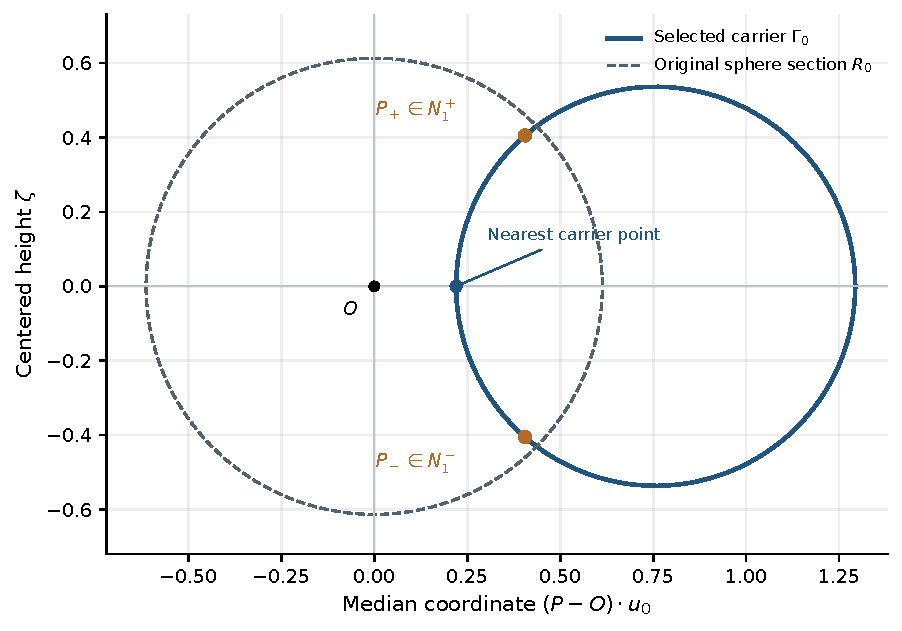
\includegraphics[width=0.78\textwidth]{figures/central_route.pdf}
\caption{The selected carrier in its median plane at width one. The dots are its actual $N_1^\pm$ contact centers; the nearest point remains distinct from $O$. The dashed circle is the original close-sphere section of radius $R_0$, a diagnostic comparison. No profile width, material wall, energetic cone or direction of flow is chosen.}\label{fig:radial}
\end{figure}

\subsection{Cut signs, complementary work and native jumps}\label{sec:regional}
For an intermediate ball let $\ell=s_0-A_{R_B}$, $r=s_0+A_{R_B}$, and define
\begin{equation}\label{eq:regionaldefinitions}
 E_B(t)=\int_\ell^r e(s,t)\dd s,\qquad
 P_L=-j(\ell,t),\quad P_R=j(r,t),\quad P_\partial=j(r,t)-j(\ell,t).
\end{equation}
The signs express outward orientation of the one-dimensional interval: increasing $s$ enters at $\ell$ and leaves at $r$. No obliquity multiplier enters this carrier account. With $H^1$ spatial fields, the cuts have traces and the weak product rule gives
\begin{equation}\label{eq:localregional}
 \dot E_B=-P_\partial+\int_{I_{R_B}}pBq\dd s,\qquad
 \dot H_N+\dot H_R=-\int_0^{L_c}pBq\dd s.
\end{equation}
For arbitrary $L^2$ carrier preparation the global port work still makes sense, but these point-cut statements do not follow from $L^2$ alone.

\begin{proposition}[Exact regional account]\label{prop:regional}
On a finite exchange or hybrid window whose endpoints are evaluated after any jump at that endpoint,
\begin{equation}\label{eq:regionalbalance}
 \begin{aligned}
 &[H_N+H_R+E_B]_{t_a}^{t_b}\\
 &\quad=\mathcal B_N(t_a,t_b)
 -\int_{t_a}^{t_b}P_\partial(t)\dd t
 -\int_{t_a}^{t_b}\int_{I_{R_B}^{c}}p(s,t)Bq(s,t)\dd s\dd t,\\
 &\mathcal B_N(t_a,t_b)=\sum_{t_a<t_n\le t_b}b_n.
 \end{aligned}
\end{equation}
For pure exchange $\mathcal B_N=0$.
\end{proposition}
\begin{proof}
Add \eqref{eq:localregional}. The integral over $I_{R_B}$ cancels only that part of the global port work, leaving the complementary integral with a minus sign. Integrate on every exchange segment, then add the native increments \eqref{eq:hybrid}; the other two stores do not jump. The stated endpoint convention includes the right endpoint's jump and excludes the left endpoint's jump.
\end{proof}

Equivalently, if a sampled window is taken from $0^-$ to $(Nh_{\rm ex})^-$, before the respective jumps, it includes $b_0,\ldots,b_{N-1}$. This is the actual native increment sum, rather than a hypothetical exchange-only baseline \cite{RX,F}.

Complete-profile containment makes the last term of \eqref{eq:regionalbalance} vanish. If containment fails, the complementary work is generally present; its sign can vary and special preparations can make it cancel. Suppressing it universally would change the account. Finally, adding $H_N$ and $H_R$ to $E_B$ is an accounting grouping: neither lumped store has thereby acquired a material location inside the diagnostic ball.

\section{Receiving before selected carrier activity}\label{sec:launch}
\subsection{The support argument for the coupled system}\label{sec:supportargument}
Define the two characteristics $w_\pm=(p\pm\rc)/\sqrt2$. Then
\begin{equation}\label{eq:characteristics}
 (w_\pm)_t\pm c(w_\pm)_s=\frac{Bq}{\sqrt2},\qquad
 j=\frac c2(w_+^2-w_-^2).
\end{equation}
For empty carrier preparation their actual coupled solution satisfies
\begin{equation}\label{eq:duhamel}
 w_\pm(s,t)=\frac1{\sqrt2}\int_0^t
 [Bq(t')](s\mp c(t-t'))\dd t'.
\end{equation}
The coefficient $q(t')$ is determined by the full exchange solution, not frozen at launch. Nevertheless, at every forcing time $t'$, the unshifted forcing $Bq(t')$ is supported in the same fixed union $\Sb$. A backward characteristic from a point at circular distance greater than $ct$ cannot meet this support during the integration interval. Therefore
\begin{equation}\label{eq:gapzero}
 d_{\rm circ}(s,\Sb)>ct\quad\Longrightarrow\quad
 w_+(s,t)=w_-(s,t)=p(s,t)=\rc(s,t)=j(s,t)=0.
\end{equation}
This is a support-gap statement relative to the entire union. Global port feedback can change the coefficients at both supports, so it is not an arbitrary system-wide locality theorem relative to just one active source point.

At the nearest point, the shortest support distance is $d_0=\eta_g-\epsc>0$. The opposite path around the seam is longer because $2\eta_g<L_c/2$. Thus the nearest-point field vanishes for $0<t<d_0/c$. This point is not exact $O$: the latter is not on the curve at all.

\begin{proposition}[Full cut-distance criterion, including Q01]\label{prop:Q01}
For either cut of half-arc $0<A<L_c/2$, the circular distance to the support union is
\begin{equation}\label{eq:cutdistance}
 d(A,\Sb)=\max\{|A-\eta_g|-\epsc,0\}
 =\begin{cases}
 \eta_g-\epsc-A,&0<A<\eta_g-\epsc,\\
 0,&\eta_g-\epsc\le A\le\eta_g+\epsc,\\
 A-\eta_g-\epsc,&\eta_g+\epsc<A<L_c/2.
 \end{cases}
\end{equation}
If this distance is positive, both cut fields and their powers vanish for $0<t<d(A,\Sb)/c$ under empty carrier preparation.
\end{proposition}
\begin{proof}
By symmetry consider the cut at offset $+A$. Its distance to the same-side closed support is the piecewise expression above. Inside the inner gap the route to the other support is longer. Beyond the outer endpoint, the route around the seam to the opposite support exceeds the same-side distance by $L_c-2A>0$; the other direct route is also longer. Thus the periodic metric does not shorten the displayed value. Apply \eqref{eq:gapzero} at both cuts.
\end{proof}

Strict containment $A>\eta_g+\epsc$ gives the enclosing-cut gap $A-\eta_g-\epsc$. It is a sufficient condition for that enclosing configuration, not a necessary condition for every delayed cut. For example, $\epsc=\eta_g/4$ and $A=\eta_g/2$ give an inner gap $d=\eta_g/4$ although containment fails. This incorporates the accepted Q01 qualification directly into the propagation argument \cite{CR}.

Zero distance does not universally force immediate activity: the port can be inactive or the solution can have special cancellation. There is, however, a useful active-port equality witness. At an outer support endpoint $A=\eta_g+\epsc$, if $q_\sigma(0)\ne0$, the outgoing characteristic has
\begin{equation}\label{eq:equalitywitness}
 w_{\rm out}(s_{\rm cut},t)
 =\frac{c\,q_\sigma(0)}{2\sqrt2\,\epsc^2}t^2+o(t^2).
\end{equation}
For sufficiently small time the incoming characteristic there is zero. To obtain \eqref{eq:equalitywitness}, the backward outgoing characteristic penetrates the tent by $c(t-t')$, where its value is $c(t-t')/\epsc^2$; integrate against $q_\sigma(t')=q_\sigma(0)+o(1)$. The outward power consequently has a positive order-$t^4$ leading term. This witness requires the active-port hypothesis and is not a universal assertion about every zero-gap cut.

\subsection{Positive receiving on the same initial interval}\label{sec:positive}
Assume now $p(0)=\rc(0)=0$, $z(0)=0$ and $f_0=f(x_0)\ne0$, with all positive parameters fixed. Then $q(0)=\eta_Nf_0$. Strong continuity of the carrier translation group in $L^2$, applied to \eqref{eq:duhamel}, yields
\begin{equation}\label{eq:launchseries}
 \begin{aligned}
 p(t)&=\eta_NtBf_0+o_{L^2}(t),&
 y(t)&=\eta_NtM_Bf_0+o(t),\\
 x(t)-x_0&=O(t^2),&
 z(t)&=\frac{\eta_N\eta_R}{2\beta_R}M_Bf_0\,t^2+o(t^2).
 \end{aligned}
\end{equation}
The last two relations follow by integrating \eqref{eq:system}; boundedness of $J_f(x)$ near launch and $y=O(t)$ gives the native estimate. Consequently
\begin{equation}\label{eq:receivergain}
 H_R(t)=\frac{\eta_N^2\eta_R^2}{8\beta_R}\norm{M_Bf_0}^2t^4+o(t^4)>0
 \quad(0<t<\delta),
\end{equation}
for some preparation-dependent $\delta>0$, since $M_B=mI_2$ and $m>0$. In the same expansion the native debit is
\begin{equation}\label{eq:nativedebit}
 H_N(0)-H_N(t)=\frac{\eta_N^2}{2}f_0^TM_Bf_0\,t^2+o(t^2).
\end{equation}
These are the inherited launch estimates \cite{RX}, with their short derivation included to exhibit that the receiver and support comparison concern the same solution.

\begin{theorem}[Receiving precedes the selected spatial activity]\label{thm:early}
Under the preceding empty-launch and nonzero-drive hypotheses, $H_R(t)>0$ while the nearest carrier point has zero field for every
\begin{equation}\label{eq:earlyinterval}
 0<t<\min\{\delta,(\eta_g-\epsc)/c\}.
\end{equation}
For any intermediate diagnostic ball with $d=d(A_{R_B},\Sb)>0$, positive receiving similarly coexists with zero fields and zero powers at both cuts on $0<t<\min\{\delta,d/c\}$. In particular this holds for strict complete-profile containment.
\end{theorem}
\begin{proof}
Intersect the positive interval in \eqref{eq:receivergain} with the zero-field intervals of \eqref{eq:gapzero} and Proposition~\ref{prop:Q01}.
\end{proof}

The theorem establishes a nonempty initial interval, not exact first-arrival times. It shows that receiver gain alone does not certify arrival at the nearest carrier point or outward passage through the chosen enclosing cuts. It does not rule out every finite central meeting region or later circulation.

\subsection{The first post-F exchange}\label{sec:postF}
The accepted cadence estimate F07 \cite{F} applies to the fixed native coefficients in \eqref{eq:native}. For $\Omega_\phi=(1,e^{i\phi},1)$ and each fixed $0<\phi\le1/100$, it gives
\begin{equation}\label{eq:F07}
 |f(F\Omega_\phi)|^2\ge
 \frac{6\Gain^2}{7}\left(\frac{97}{100}\right)^2
 \left(\frac{284971}{300000}\right)^2\sin^2\phi>0.
\end{equation}
If carrier and receiver are empty before that native step, they remain empty immediately after it. Theorem~\ref{thm:early} therefore applies to the first exact exchange, with time measured from that post-jump state, on
\begin{equation}\label{eq:postFinterval}
 0<t<\min\{h_{\rm ex},\delta(\phi,\text{fixed parameters}),d/c\},
\end{equation}
where $d$ is the nearest-point distance or a positive cut distance. The parameter tuple is fixed before choosing the phase, and the result is phasewise. No uniform positive interval over all phases, later preloaded exchange stages or exact first-arrival claim is inferred.

\section{Uniform separation from the six central openings}\label{sec:separation}
\subsection{The individual-hull envelope}\label{sec:hulls}
For each of the six boundaries define its individual convex enclosure
\begin{equation}\label{eq:hulls}
 \Hull_k^\sigma=\operatorname{conv}(G_k^\sigma).
\end{equation}
It is the triangle formed by that boundary's elbow and two tips. This is a mathematical bounding set, not a declaration that an opening is a filled material aperture. Each upper hull lies in $h_g\le\zeta\le H_0$; each lower hull lies in $-H_0\le\zeta\le-h_g$.

For any spatial point let $r_\perp(P)=\norm{P_h}$ be its cylindrical radius about the axis through $O$, and set
\begin{equation}\label{eq:separator}
 \Phi(P)=r_\perp(P)-\frac35|\zeta(P)|,\qquad
 D_* =\sqrt{10-6\sqrt2},\qquad L_* =\frac{\sqrt{34}}5.
\end{equation}
Since $J_\perp^T=-J_\perp$ and $J_\perp^TJ_\perp=I$,
\begin{equation}\label{eq:similarity}
 A_{\tau_g}^TA_{\tau_g}
 =\left(1+\frac{\tau_g^2}{r_g^2}\right)I,\qquad
 \sqrt{1+\tau_g^2/r_g^2}\le\sqrt{1+h_g^2/r_g^2}=D_*.
\end{equation}
Every elbow therefore has cylindrical radius at most $D_*a_g$, and every tip at most $D_*r_g$. Reflection preserves both radius and absolute height. The exact vertex inequalities are
\begin{equation}\label{eq:vertexbounds}
 D_*a_g-\frac35h_g<\frac3{50},\qquad
 D_*r_g-\frac35H_0<\frac3{50}.
\end{equation}
Appendix~\ref{sec:arithmetic} gives rational certificates for these comparisons.

\begin{proposition}[Uniform individual-hull envelope]\label{prop:hullenvelope}
For every $k$, sign $\sigma$, admitted $\tau_g$ and hand,
\begin{equation}\label{eq:envelope}
 \Phi(Q)\le\frac3{50}\qquad(Q\in\Hull_k^\sigma).
\end{equation}
\end{proposition}
\begin{proof}
On either fixed-sign height halfspace, $\Phi$ is a norm minus a linear function, hence convex. Each individual hull stays in one such halfspace. Convexity and \eqref{eq:vertexbounds} bound every convex combination of its three vertices. More explicitly, if $t$ is the total weight of the two tips, then
\begin{equation}\label{eq:hullinterpolation}
 |\zeta(Q)|=(1-t)h_g+tH_0,\qquad
 r_\perp(Q)\le D_*[(1-t)a_g+tr_g],\quad 0\le t\le1.
\end{equation}
Subtracting three fifths of the height makes the estimate a convex combination of the two vertex bounds. Both endpoints of the static parameter range are included.
\end{proof}

One cannot replace the six individual hulls by their combined convex hull: $\Phi$ is not globally convex. At $\tau_g=0$, an upper and lower tip at the same horizontal position $r_ge_{2k}$ have midpoint $(r_ge_{2k},0)$, with $\Phi=r_g>3/50$, although each tip has $\Phi=r_g-3/10<3/50$. This is why the fixed-sign condition is essential.

\subsection{The carrier separator and a Euclidean bound}\label{sec:clearance}
Because $K_c/\RG=(2+\sqrt3)/\sqrt7>1$, the coefficient $K_c+\RG\cos\theta$ never changes sign. For every geometric circle,
\begin{equation}\label{eq:cylindrical}
 r_\perp(\Gamma_j(\theta))=K_c+\RG\cos\theta,\qquad
 \zeta(\Gamma_j(\theta))=\RG\sin\theta.
\end{equation}
This cylindrical radius differs from the radial distance $D$ in \eqref{eq:radial}. Cauchy--Schwarz on $(\cos\theta,|\sin\theta|)$ gives
\begin{equation}\label{eq:carriergap}
 \Phi(\Gamma_j(\theta))\ge K_c-L_*\RG,
 \qquad \Delta_*:=K_c-L_*\RG-\frac3{50}>0.
\end{equation}
The strict positivity is certified below. The scalar-function gap is not yet a spatial distance. For arbitrary points, including the axis and opposite height signs, reverse triangle inequalities give
\begin{equation}\label{eq:lipschitz}
 \begin{aligned}
 |\Phi(P)-\Phi(Q)|
 &\le |r_\perp(P)-r_\perp(Q)|+\tfrac35\big||\zeta(P)|-|\zeta(Q)|\big|\\
 &\le\norm{P_h-Q_h}+\tfrac35|\zeta(P)-\zeta(Q)|\\
 &\le L_*\norm{P-Q}.
 \end{aligned}
\end{equation}
This is a global Lipschitz estimate and uses no differentiability at the norm's singular points.

\begin{theorem}[Uniform six-opening clearance]\label{thm:separation}
Under the common geometric scaling of all centered coordinates and the static parameter by $\wh>0$, every geometric circle and every individual hull satisfy, for all admitted $\tau_g$, both hands, all $j,k$ and $\sigma$,
\begin{equation}\label{eq:distance}
 \operatorname{dist}(\Gamma_{j,\wh},\Hull_{k,\wh}^{\sigma,\mathrm{hand}})
 \ge\wh\frac{\Delta_*}{L_*}
 >\frac{23107}{389000}\wh
 >\frac{297}{5000}\wh.
\end{equation}
The same bound holds with the actual broken boundary $G_{k,\wh}^{\sigma,\mathrm{hand}}$ in place of its hull.
\end{theorem}
\begin{proof}
At width one, \eqref{eq:envelope} and \eqref{eq:carriergap} imply $\Phi(P)-\Phi(Q)\ge\Delta_*$ for every circle point $P$ and hull point $Q$. Equation~\eqref{eq:lipschitz} gives $\norm{P-Q}\ge\Delta_*/L_*$. Taking the infimum proves the non-strict estimate. The rational bounds in Appendix~\ref{sec:arithmetic} establish
\begin{equation}\label{eq:coarsegap}
 \Delta_*>\frac{69321}{1000000},\qquad L_*<\frac{1167}{1000},\qquad
 \frac{69321/1000000}{1167/1000}=\frac{23107}{389000}>\frac{297}{5000}.
\end{equation}
All divisions involve positive quantities. The subset $G\subset\Hull$ gives the boundary statement. Common scaling multiplies distances, $r_\perp$, $|\zeta|$ and the gap by $\wh$ while leaving $\tau_g/r_g$ and $L_*$ unchanged.
\end{proof}

The exact conservative expression $\Delta_*/L_*$ is approximately $0.06097180165653555$ at width one. It is not the actual minimum distance or an optimized clearance: saturation of the circle separator does not imply that any hull point saturates its envelope at a closest pair. The rational conclusion in \eqref{eq:distance} is independent of this decimal display.

\begin{figure}[htbp]\centering
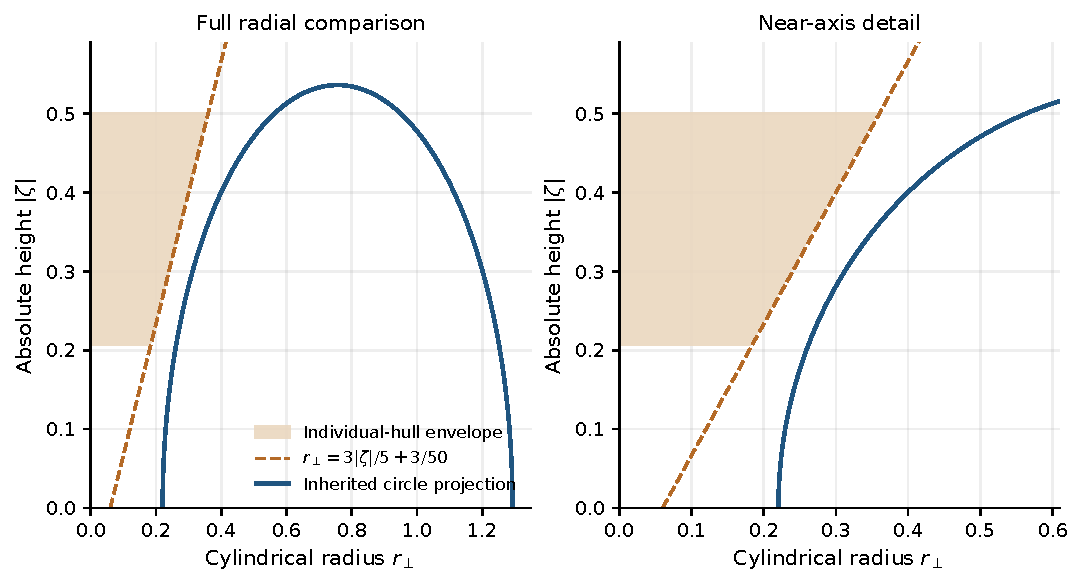
\includegraphics[width=\textwidth]{figures/six_opening.pdf}
\caption{Radial/absolute-height projection at width one: the full comparison (left) and a close view (right). The shading bounds each individual $G$ hull using \eqref{eq:hullinterpolation}; it is not a physical aperture. The dashed separator is $r_\perp=3|\zeta|/5+3/50$. The circle lies strictly on its exterior side for all angles. Rotation and full reflection leave these projected quantities unchanged. Sampled plotting points illustrate the exact inequalities; they do not establish the uniform theorem.}\label{fig:separation}
\end{figure}

\Needspace{9\baselineskip}
\begin{corollary}[No direct crossing parameter]\label{cor:empty}
For every circle in the unchanged registration,
\begin{equation}\label{eq:empty}
 \Gamma_j^{-1}(G_k^{\sigma,\mathrm{hand}})=\varnothing,
 \qquad \Gamma_j^{-1}(\Hull_k^{\sigma,\mathrm{hand}})=\varnothing.
\end{equation}
The spatial images $\gamma_0(S_\pm)$ of the finite source/loading supports obey the same lower distance bound.
\end{corollary}
\begin{proof}
An intersection would have distance zero, contradicting Theorem~\ref{thm:separation}. The support images are subsets of $\Gamma_0$.
\end{proof}

Changing arclength width along this curve cannot create off-curve incidence. The theorem covers a future aperture \emph{if} it lies wholly within its individual hull, but no such aperture has been adopted. An unspecified thick tube, nonplanar spanning surface or relative translation or rescaling of one object requires a separate analysis. The common-width result is geometric and does not assign physical units.

\section{Transport, information and direction labels}\label{sec:transport}
\subsection{Which work is already defined?}\label{sec:Gtransport}
A literal one-dimensional carrier crossing of a spatial set requires an arclength parameter whose image belongs to that set, before one can ask about transversality or outward orientation. Corollary~\ref{cor:empty} supplies no such parameter for any central $G$ boundary or individual hull. The host $N_1^\pm$ contacts do have the parameters $s_\pm$, with signed outgoing powers $-j(s_+,t)$ and $+j(s_-,t)$ for their intervening interval. Diagnostic-ball cuts have their own power $j(r,t)-j(\ell,t)$. Distributed per-port supply and loading, $\eta_Nf_\sigma y_\sigma$ and $\eta_Rz_\sigma y_\sigma$, are profile-integrated work, not point-cut powers.

These distinctions prevent relabeling any of those quantities as transport through the six central openings. The existing equations specify no six-aperture spatial flux, receiving map or matched loading term. An empty sum of direct intersections would record geometric nonintersection; it would not define a physical aperture flux and calculate it as zero.

The difference between two port inputs and six boundary labels is not a dimension-based impossibility theorem. Two scalars can have six correlated outputs, and the carrier also has spatial and temporal histories. What is absent is a justified spatial and energetic registration, not the abstract possibility of writing a map. No allocation matrix is selected here.

\subsection{What exchange histories retain about phase}\label{sec:phase}
Let common rephasing act on the native real coordinates by
\begin{equation}\label{eq:Q}
 Q_\theta(a,b)=(\cos\theta\,a-\sin\theta\,b,\ \sin\theta\,a+\cos\theta\,b).
\end{equation}
Bilinearity and antisymmetry of the cross product give $f(Q_\theta x)=f(x)$. Differentiating this identity and using orthogonality yields
\begin{equation}\label{eq:equivariance}
 J_f(Q_\theta x)=J_f(x)Q_\theta^T,\qquad
 -J_f(Q_\theta x)^Ty=Q_\theta[-J_f(x)^Ty].
\end{equation}
Thus the native exchange vector field is equivariant, and the external equations see exactly the same $q$. Uniqueness of the coupled solution gives the following result.

\begin{proposition}[Exchange common-phase information]\label{prop:phase}
With identical initial $p,\rc,z$ and native initial states related by $Q_\theta$, the exchange trajectories have identical complete histories of $p,\rc,z$, while their native histories remain related by $Q_\theta$. Hence an outlet rule that genuinely distinguishes such states cannot be reconstructed solely from those exchange histories.
\end{proposition}
\begin{proof}
Apply $Q_\theta$ to the native component of one solution and leave its external components fixed. Equations~\eqref{eq:system} and \eqref{eq:equivariance} show that this is a solution with the rephased initial data. Uniqueness identifies it with the second solution. If a function of the common external history represented two different outlet values, it would take two values on the same input, a contradiction.
\end{proof}

This obstruction is conditional on genuine common-phase sensitivity. It does not require every possible outlet rule to have that sensitivity, and does not say all relative-phase information is lost. For the native map $F$, common-phase equivariance holds when all prestage entries are nonzero, since phase differences are preserved modulo $2\pi$. At a zero prestage, $\operatorname{Arg}_0(0)=0$ does not shift with the other arguments and may alter neighboring kicks; no unrestricted singular-prestage extension is used. Likewise, the earlier reduced-coordinate reconstruction for autonomous $F$ histories \cite{AX} is not automatically a reconstruction rule during coupled exchange or arbitrary hybrid evolution, even if the coordinates remain in its original domain.

\subsection{Ports are not propagation senses}\label{sec:labels}
The port sign $\sigma=\pm$ names the upper or lower spatial contact/profile. The sign on $w_\pm$ names increasing or decreasing arclength propagation in \eqref{eq:characteristics}. Each source profile occurs in both characteristic equations. The contact tangent identities $\gamma'(s_+)=-n_+$ and $\gamma'(s_-)=n_-$ do not insert new signs in the raw drive \eqref{eq:drive}. Nor does the sign of a source coefficient alone fix the power $j=c(w_+^2-w_-^2)/2$. Identifying upper with outward, lower with inward, or the two ports with the two characteristic senses would therefore add an unsupported direction rule.

\subsection{Conditional off-carrier observation}\label{sec:C6}
The inherited C6 observation \cite{CC} is defined at a fixed point $X$ off the carrier, with supplied retarded history, a fixed observation frame and independent positive $c_e,g_o$. With $d_X(s)=\norm{X-\gamma_0(s)}$ and $\widehat t(s)=\gamma'_0(s)$, its scalar and vector components are
\begin{equation}\label{eq:C6}
 \begin{aligned}
 U(X,t)&=\frac{g_o}{4\pi}\int_0^{L_c}
 \frac{p(s,t-d_X(s)/c_e)}{d_X(s)}\dd s,\\
 V_{\rm ext}(X,t)&=\frac{g_o}{4\pi}\int_0^{L_c}
 \frac{\rc(s,t-d_X(s)/c_e)\widehat t(s)}{d_X(s)}\dd s.
 \end{aligned}
\end{equation}
The vector can be resolved in the declared orthonormal observation frame. Continuous-in-time $H^1$ histories give the required pointwise representatives; the full retarded history must actually be supplied. For a fixed point on any specified $G$ boundary or individual hull in the width-one static configuration used in \eqref{eq:C6}, Theorem~\ref{thm:separation} guarantees $d_X(s)>297/5000$. For a commonly scaled carrier and central geometry, with the arclength interval scaled accordingly, the corresponding distance is strictly greater than $297\wh/5000$. It therefore supplies the geometric off-carrier condition and a denominator bounded away from zero, but does not supply the history. A moving $X(\tau_g(t))$ is a different problem: the admitted static parameter is not time.

No term in \eqref{eq:C6} loads the carrier or advances the receiver. The encoded tangent field $\rc\widehat t$ is not the scalar cut flux $j$ or a declared ambient energy-current density, and $|U|^2+\norm{V_{\rm ext}}^2$ is not an inherited receiving store. The C6 observation can therefore be evaluated conditionally at an opening without establishing transport or energetic loading there.

The macro observation has a further distinct role. Under its declared axial placement, $A\cos(3(\theta_{\rm obs}-\ell))(\cos\theta_{\rm obs},\sin\theta_{\rm obs},1)$ lies on a double cone. Staged $Z$ adds raw chirality and need not stay on that cone \cite{CG,AX}. Its amplitude, observation clock and placement define a readout, not an energetic emission law. The outer host, refined central surface, intended tight toroid, optional tube, original close sphere and extended-line sphere retain their separate definitions.

\section{Synthesis and the completed correspondence boundary}\label{sec:synthesis}
The two results answer complementary questions. The temporal result shows that a receiver can gain storage through the registered local interfaces before the selected carrier travel events. The spatial result shows that those same interfaces remain separated from the six central boundaries and their individual convex enclosures. Both statements coexist with exact reciprocal work, radial approach and recession along the carrier, and the positioned stationary-axis dictionary.

To turn the intended route into a further transport model, a spatial registration must supply three connected ingredients:
\begin{enumerate}
\item the actual set receiving or being crossed, together with orientation and measure when a surface flux is intended;
\item a map from the existing state, and any explicitly introduced additional state, to the transported or loaded quantity on that set;
\item the matching work and stock relation, so that receiving and the associated carrier/native debit are consistently accounted for.
\end{enumerate}
A measurement-only construction instead needs a declared observation interpretation and should not be called an energetic load. These requirements identify the missing connection without choosing a new aperture closure, connector, receiver, thickness, clock or efficiency target.

The candidate already has reciprocal feedback and a reversible receiver. Same-solution native credit, exchange-only capacity-sized receiving/recovery, and the scoped cadence results are completed parts of the inherited programme \cite{RX,RR,F}. Historical source sentences describing these as absent or open do not control the present status. Later receiving/recovery after native steps and preload remains a separate question; it is not supplied by the empty-launch theorem here.

Local exchange can participate in a later larger circuit, including transfer elsewhere. The present results do not force a choice between those possibilities. They complete the correspondence assessment at the retained definitions: receiving alone does not certify the specified travel, and central-opening transport cannot be obtained by renaming the existing host contacts. Further spatial connection is subsequent research, with no new strict order imposed on the other retained directions.

The mathematical basis is the accepted C01--C05 investigation with Q01 and the accepted S01--S05 investigation \cite{CR,SO}. The central-route record contains eight independently written algebra groups with the more limited corroboration described by its GPT acceptance. The six-opening record contains six independent exact-check groups and a later GPT replay of those same six groups. The replay is not six additional independent proofs, and it is not a full replay of the central-route suite. The arguments above supply the support, trace, convexity, Lipschitz and interpretation steps for which arithmetic checks alone would not suffice. This manuscript preparation uses the retained evidence, without a new scientific-suite execution or trajectory simulation. Its claim ledger and document build/inspection records accompany the editable edition; manuscript review remains separate from acceptance of its mathematical foundations.

\appendix
\section{Exact arithmetic and evidence guide}\label{sec:arithmetic}
The coarse enclosures below are sufficient for the uniform rational clearance:
\begin{equation}\label{eq:radicalintervals}
 \begin{array}{rcl@{\qquad}rcl}
 14142/10000&<\sqrt2<&14143/10000,&17320/10000&<\sqrt3<&17321/10000,\\
 24494/10000&<\sqrt6<&24495/10000,&26457/10000&<\sqrt7<&26458/10000.
 \end{array}
\end{equation}
Each interval is certified by squaring its positive rational endpoints. Put $D_u=1231/1000$, $a_u=(1-14142/20000)/2$, $h_l=(14142/10000-1)/2$, and $r_u=17321/60000$. Then
\begin{equation}\label{eq:vertexcertificate}
 \begin{aligned}
 D_u^2-(10-6\cdot14142/10000)&=561/1000000>0,\\
 \frac3{50}-(D_ua_u-\tfrac35h_l)&=79601/20000000>0,\\
 \frac3{50}-(D_ur_u-\tfrac3{10})&=277849/60000000>0.
 \end{aligned}
\end{equation}
These certify \eqref{eq:vertexbounds} in the correct monotone directions. From the same intervals and $\RG=\sqrt7K_c/(2+\sqrt3)$,
\begin{equation}\label{eq:gapcertificate}
 \begin{gathered}
 \frac{45401}{60000}<K_c<\frac{45403}{60000},\qquad
 \RG<\frac{600636287}{1119600000}<\frac{537}{1000},\qquad
 L_*<\frac{1167}{1000},\\
 \Delta_* >\frac{756}{1000}-\frac{1167}{1000}\frac{537}{1000}-\frac3{50}
 =\frac{69321}{1000000},\\
 \frac{69321}{1000000}-\frac{297}{5000}\frac{1167}{1000}
 =\frac3{2500000}>0.
 \end{gathered}
\end{equation}
For example $(1167/1000)^2-34/25=1889/1000000>0$ proves the $L_*$ bound. These strict rational margins are the certificates used in Theorem~\ref{thm:separation}; no plotted samples enter them.

The radial comparisons \eqref{eq:closemargins} can also be checked directly with these coarse intervals. With $K_l=45401/60000$, $K_u=45403/60000$, put $a_u'=K_u/(1+17320/20000)$ and $R_l=(26457/10000)K_l/(2+17321/10000)$. Integer cross-multiplication gives
\begin{equation}\label{eq:radialcertificate}
 \begin{aligned}
 \frac{13}{12}-\frac{14143}{20000}-2(a_u')^2&>\frac4{100},\\
 K_l^2+R_l^2+\frac{2K_lR_l}{7}
 -\left(\frac{13}{12}-\frac{14142}{20000}\right)&>\frac{59}{100}.
 \end{aligned}
\end{equation}
The accepted central-route record retains finer rational enclosures as well. These weaker displayed bounds make the signs used here auditable without decimal approximations.

\begin{table}[htbp]\centering\small
\caption{Accepted claims and their principal locations in this manuscript. The companion ledger supplies exact source paths, labels and recorded equation/page numbers.}\label{tab:claims}
\begin{tabularx}{\textwidth}{@{}lX@{}}\toprule
Accepted item & Manuscript location and content\\\midrule
C01, S01 & Section~\ref{sec:model}: native registration, positioned axes, finite $N$, actual $G$, profiles, exchange and F-first ordering.\\
C02 & Proposition~\ref{prop:ball} and \eqref{eq:widthceiling}: radial preimages, complete profiles and close-sphere ceiling.\\
C03 & Proposition~\ref{prop:regional}: oriented cuts, complementary work, regularity and jump counting.\\
C04 & Theorem~\ref{thm:early}, \eqref{eq:equalitywitness} and \eqref{eq:postFinterval}: coupled empty launch and first post-F scope.\\
Q01 & Proposition~\ref{prop:Q01}: full cut distance, inner-gap witness and active-port qualification.\\
S02 & Proposition~\ref{prop:hullenvelope}: individual fixed-sign hulls over the whole static family.\\
S03 & Theorem~\ref{thm:separation} and Corollary~\ref{cor:empty}: uniform clearance, common scaling and empty preimages.\\
C05 & Proposition~\ref{prop:phase} and Sections~\ref{sec:phase}--\ref{sec:labels}: common-phase information and propagation labels.\\
S04 & Sections~\ref{sec:Gtransport}, \ref{sec:C6}: direct crossings versus undefined aperture flux and unloaded observation.\\
S05 & Section~\ref{sec:synthesis}: missing registration, current completion status and subsequent research.\\\bottomrule
\end{tabularx}
\end{table}

The companion package preserves both complete acceptance archives and readable proof/disposition records. Its source registry records 65 retained source, context, acceptance, figure and precedent files, including SHA-256 and available Git blob identities. The common later repository reading checkpoint is \texttt{c3ee366bd6195bd7fa77efd0321214af4c2dc173}; retained older snapshots keep their own recorded identities. Immutable links in the bibliography locate editions; the exact per-file records identify the bytes actually consulted. The source paths and labels in the companion claim ledger take precedence over similarly named labels in different papers.

\section{Editorial notation crosswalk}\label{sec:crosswalk}
The renamings in Table~\ref{tab:notation} separate quantities whose source symbols collided. They introduce no new physical assumption. In particular $R_B$ is a diagnostic ball radius, not a cylindrical coordinate; $r_\perp$ is a cylindrical coordinate, not a diagnostic region size.

\small
\begin{longtable}{@{}>{\raggedright\arraybackslash}p{0.39\textwidth}>{\raggedright\arraybackslash}p{0.29\textwidth}>{\raggedright\arraybackslash}p{0.25\textwidth}@{}}
\caption{Source-to-manuscript notation.}\label{tab:notation}\\
\toprule Meaning & Source notation & This paper\\\midrule\endfirsthead
\toprule Meaning & Source notation & This paper\\\midrule\endhead
Diagnostic ball radius & CR $\rho$ & $R_B$\\
Cylindrical radius about $O$ axis & SO $\rho(P)$ & $r_\perp(P)$\\
Receiver state & $z\in\R^2$ & $z$\\
Centered spatial height & geometric $z,w,\zeta$ & $\zeta(P)$\\
Common host width & SO $w$ & $\wh$\\
Carrier characteristics & $w_\pm$ & $w_\pm$\\
Native source Jacobian & $J=D_xf$ & $J_f$\\
Horizontal quarter-turn & $J(X,Y)=(-Y,X)$ & $J_\perp$\\
Static geometry parameter & $\tau$ & $\tau_g$\\
Exchange time/integration dummy & $t,\tau$ & $t,t'$\\
Geometry half-height & CG $h$ & $h_g$\\
Exchange dwell & hybrid $h$ & $h_{\rm ex}$\\
Contact arclength offset & $\eta,\eta_{\rm geom},\eta_g$ & $\eta_g$\\
Native/receiver multipliers & $\eta,\kappa$ or $\eta_N,\eta_R$ & $\eta_N,\eta_R$\\
Circle offset/plane constant & PG $\kappa$, CR $K_c$ & $K_c$\\
Circle radius & $R_c,R_\Gamma$ & $\RG$\\
Raw source gain & $G$ & $\Gain$\\
Central broken boundaries & $G_k^\sigma$ & $G_k^\sigma$\\
Support union & $S$ & $\Sb$\\
Centered MINUS reflection & $S$ & $S_{\rm ref}$\\
Angle and arclength curves & $\Gamma_j(\theta),\Gamma(s)$ & $\Gamma_j(\theta),\gamma_j(s)$\\
Lower vertices/circle center & $B_i,B_j$ & $B_i$; circle center written $O+K_cu_j$\\
\bottomrule
\end{longtable}
\normalsize

\clearpage
\begin{thebibliography}{9}
\raggedright
\bibitem{PG} H.~Frímann Halldórsson,
\emph{Paired-Gap Geometry and Toroidal Observation Maps for the Folded Tri-Octagon}, v0.1.1 (2026).
\href{https://github.com/pzychozen/trioctagon-physics/tree/c3ee366bd6195bd7fa77efd0321214af4c2dc173/SRG_REDISCOVERY/PAPERS/PAIRED_GAP_GEOMETRY_OBSERVATION/publication/v0.1.1}{Immutable edition at the reading checkpoint}.
Retained geometry source: carrier circle, finite host contacts and original close sphere.

\bibitem{AX} H.~Frímann Halldórsson,
\emph{Phase Reconstruction and Stationary Support Axes in the Tri-Octagon Map}, v0.1 (2026).
\href{https://github.com/pzychozen/trioctagon-physics/tree/c3ee366bd6195bd7fa77efd0321214af4c2dc173/papers/PHASE_RECONSTRUCTION_AND_STATIONARY_SUPPORT_AXES/publication/v0.1}{Immutable edition at the reading checkpoint}.
Retained setting, spatial, observations and rotation sources: positioned axes, decoder and reconstruction scope.

\bibitem{CG} H.~Frímann Halldórsson,
\emph{Central Geometry, Z Readouts, and Chiral Response in the Tri-Octagon Model}, v0.3 (2026).
\href{https://github.com/pzychozen/trioctagon-physics/tree/c3ee366bd6195bd7fa77efd0321214af4c2dc173/papers/CENTRAL_GEOMETRY_Z_CHIRAL_RESPONSE/publication/v0.3}{Immutable edition at the reading checkpoint}.
Retained manuscript: static central family, full reflection, six broken boundaries and observation geometry.

\bibitem{CC} H.~Frímann Halldórsson,
\emph{Native Intensity Accounting and Conditional Carrier Crossings in the Tri-Octagon Model}, v0.1 (2 November 2026).
\href{https://github.com/pzychozen/trioctagon-physics/tree/c3ee366bd6195bd7fa77efd0321214af4c2dc173/papers/NATIVE_INTENSITY_AND_CONDITIONAL_CARRIER_CROSSINGS/publication/v0.1}{Immutable edition at the reading checkpoint}.
Retained geometry, carrier, readouts and conclusion sources; C6 is the conditional unloaded observation.

\bibitem{RX} H.~Frímann Halldórsson,
\emph{A Reciprocal Chiral Exchange Extension of the Tri-Octagon Model}, v0.1 (2026).
\href{https://github.com/pzychozen/trioctagon-physics/tree/273b1a6faaab19ea58748d00576439166eeef9ab/papers/RECIPROCAL_CHIRAL_EXCHANGE/publication/v0.1}{Immutable published edition}.
Retained candidate, power, accounts, well-posedness, activity, capacity and hybrid sources; the global theorem supplies the exchange regularity used here.

\bibitem{RR} H.~Frímann Halldórsson,
\emph{Capacity-Sized Receiving and Native Recovery in the Reciprocal Chiral Exchange Candidate}, v0.1 (2026).
\href{https://github.com/pzychozen/trioctagon-physics/tree/34bf6c6e4e18adcc177ac700359fda16cf4d772d/papers/NATIVE_CAPACITY_RECEIVING_RECOVERY/publication/v0.1}{Immutable published edition}.
Retained model and interpretation sources: fixed-yaw exchange and the current receiving/recovery scope.

\bibitem{F} H.~Frímann Halldórsson,
\emph{Native Stepping and Exchange Cadence in the Reciprocal Chiral Exchange Candidate}, v0.1 (2026).
\href{https://github.com/pzychozen/trioctagon-physics/tree/c3ee366bd6195bd7fa77efd0321214af4c2dc173/papers/NATIVE_F_STEPPING_EXCHANGE_CADENCE/publication/v0.1}{Immutable edition at the reading checkpoint}.
The retained accepted investigation and GPT acceptance supply F01, F07--F08 and the scoped cadence conclusions; native source text separately fixes the update conventions.

\bibitem{CR} H.~Frímann Halldórsson, with GPT formulation and Codex independent investigation,
\emph{Central-route correspondence}, internal research record, 9 November 2026.
Accepted proof C01--C05, claim ledger and GPT review, including Q01, preserved in the companion package under \sourcepath{inputs/accepted/central_route/}. This is an accepted investigation, not an earlier published edition of the present manuscript.

\bibitem{SO} H.~Frímann Halldórsson, with GPT formulation and Codex independent investigation,
\emph{Six-opening transport correspondence}, internal research record, 9 November 2026.
Accepted proof S01--S05, claim/source ledger and GPT review, preserved under \sourcepath{inputs/accepted/six_opening/}. The unchanged acceptance archive includes the independent exact checks and the later replay of those same six groups.
\end{thebibliography}

\end{document}
